\documentclass[11pt,a4paper]{article}

\usepackage[utf8]{inputenc}
\usepackage[spanish]{babel}

\usepackage{amsmath, amssymb, amsthm}
\usepackage{mathrsfs}
\usepackage{appendix}

\usepackage{hyperref}
\usepackage{captdef}

\usepackage{psfrag}
\usepackage{graphicx}
\usepackage{subfig}
\usepackage{color}
\usepackage{multicol} 

%\usepackage{fancyhdr}
%\pagestyle{fancy}
%\fancyhf{}

\newcommand{\C}{\mathscr{C}} 

\usepackage{cancel}
\usepackage[usenames,dvipsnames,svgnames,table]{xcolor}
\usepackage[left=2cm,right=2cm,top=2cm,bottom=2cm]{geometry}
\usepackage{caption}
%\usepackage{subcaption}
%\renewcommand{\baselinestretch}{1.5}

\usepackage{hyperref}
%\usepackage[hidelinks]{hyperref} 
\hypersetup{
    colorlinks=true,
    linkcolor=blue,
    filecolor=magenta,      
    urlcolor=cyan,
    }

\begin{document}
\thispagestyle{empty}

\includegraphics[height=3.5cm]{escudoCiencias.pdf}
\vspace{-3.8cm}
\begin{flushright}
\hspace{4cm}
{\Large\textbf{El modelo de Ising para estudiar el comportamiento de un ferromagneto.}\vspace{0.2cm}

Laboratorio de Física Contemporánea II}
\vspace{0.3cm}\\
\begin{large}Autor: Rodrigo Vega Vilchis.\end{large}\\
\begin{footnotesize}
Correo: rockdrigo6@ciencias.unam.mx\\
\hspace{2.05cm}{\color{white}.}\\
\end{footnotesize}
\vspace{0.1cm}
\begin{large}Profesor: Ricardo Martín Hernández Flores\\
Ayudante: Alberto del Ángel Medina\\
25 de abril, 2022\end{large}\\
\end{flushright}
%\vspace{.4cm}
 \hrule height1pt\vspace{.5cm}
\begin{abstract}
En este trabajo se utilizó el algorítmo de Metrópolis-Montecarlo para estudiar el comportamiento de un ferromagneto en distintos ámbitos: se analizó el comportamiento de la energía y magnetización para una temperatura previa y posterior a la temperatura crítica; se se analizaron 6 configuraciones de espines a tres temperaturas menores a la críticas y tres mayores o iguales a la misma. Por último se analizaron cuatro cantidades observables: energía por sitio, magnetización por sitio, calor específico y susceptibilidad magnética. La transición de fase al ser de segundo orden, presenta discontinuidades en las últimas dos cantidades.
\end{abstract}


\section{Introducción}

El modelo de Ising fue implementado por primera vez por el físico Wilhelm Lenz en 1920 y resuelto por su alumno Ernst Ising, es un modelo que carga con una importancia que abarca desde la descripción del comportamiento de un ferromagneto, su transición de fase dada una temperatura crítica y algunas otras aplicaciones que se extienden al modelado de problemas sociales y/o biológicos en donde intervienen interacciones no-lineales en un conjunto denso de individuos\footnote{cfr. Barradas-Bautista D, Alvarado-Mentado
M, Agostino M, Cocho G (2018) Cancer growth
and metastasis as a metaphor of Go gaming: An
Ising model approach. PLoS ONE 13(5):
e0195654. https://doi.org/10.1371/journal.
pone.0195654}.\\
\\
Los materiales en general tienen la fortuna de estar caracterizados por dos propiedades electromagnéticas importantes que se relacionan entre sí: la \textit{susceptibilidad magnética} que no es más que un parámetro adimensional que nos dice qué tan susceptible es un material de ser magnetizado por un campo magnético externo $\vec{H}_{Ext}$\footnote{donde consideramos que el campo magnético es: $\vec{H}=\vec{B}-4\pi\vec{M}$ y la susceptibilidad magnética es: $\vec{M}=\chi_m\vec{H}$}. Por otro lado, el campo de inducción magnética $\vec{B}$ está definido en términos de la \textit{permeabilidad magnética}\footnote{se define como: $\vec{B}=\mu\vec{H}$}, definida como la capacidad de los materiales para afectar y ser afectados por campos magnéticos. En esta dirección, existen tres posibles casos para el valor de la permeabilidad magnética $\mu$ que dan origen a los materiales: \textbf{diamagnéticos} ($\mu<1$), \textbf{paramagnéticos} ($\mu>1$) y \textbf{ferromagnéticos} ($\mu\gg1$).\\
\\
Los diamagnéticos son aquellos materiales cuyos espines que lo conforman se alinean en dirección contraria  a un campo magnético incidente. Contrario a éstos materiales están los paramagnéticos, en donde los espines que lo conforman se alinean en la misma dirección de un campo magnético externo pero con la condición de que al alejarlo del material, éste regresará a su estado inicial. Finalmente los ferromagnéticos son aquellos materiales que poseen \textit{dominios magnéticos}\footnote{Son regiones en donde varios momentos magnéticos quedan confinados y alineados entre sí} que al imponerles un campo magnético suficientemente fuerte, se alinean paralelamente a este campo y después de la exposición quedan alineados en dicha dirección.\\
\\

Para modelar uno de los materiales descritos (específicamente un ferromagneto) consideramos una red cristalina en donde es necesario conocer las interacciones que existen a nivel atómico: tales como las electrostáticas, entre electrones y iones de valencia etc. Todas ellas las podemos remitir a interacciones entre átomos: determinando las interacciones que genera el campo magnético del i-ésimo átomo de la red con un j-ésimo átomo vecino. Con éstos recursos y la posible presencia de un campo magnético  externo $\vec{H}$ es posible armar un hamiltoniano de interacciones que nos determine la energía del sistema, la cual está dada por
\begin{equation}\label{eq:Energia}
E=-J\sum_{\langle ij\rangle}s_is_j-H\sum_i s_i
\end{equation}
donde la notación $\langle ij\rangle$ indica la suma sobre los primeros vecinos de la red, $s_k=\pm1$ indica espines arriba o abajo de acuerdo al signo, $J$ es una constante que contiene todos los coeficientes del campo y el momento dipolar magnéticos; además si $J>0$, los spines tienden a orientarse de manera paralela ($\uparrow\uparrow$ o $\downarrow\downarrow$), mientras que con $J<0$ los espines se alinean de forma antiparalela ($\uparrow\downarrow$). Sin embargo a nosotros nos interesa el caso $J>0$ que corresponde a la descripción de un ferromagneto.\\
\\
Estos materiales pueden ser vistos como sistemas termodinámicos que dependen fuertemente de la temperatura a la que estén. Es posible observar como un imán puede dejar de serlo al aplicarle calor hasta una cierta temperatura crítica, incrementando la entropía del sistema y desalineando los dominios magnéticos del ferromagneto pasando ahora a un paramagneto. Esta transición de fase está relacionada con la discontinuidad en la segunda derivada de la energía con respecto del campo magnético; la primera derivada es la magnetización y esa si es continua, pero la segunda es la susceptibilidad magnética que según la Ley de Curie-Weiss
\begin{equation}\label{eq:Curie-Wiess}
\chi_m=\frac{C}{T-T_C}
\end{equation}
presenta una notable discontinuidad en la temperatura de Curie, la cual es distinta para cada material aunque en ferromagnetos es muy alta. Para poder darle solución al modelo se puede partir de la función de partición del ensamble canónico, sin embargo al realizar los cálculos para redes grandes (por ejemplo de $100\times100$), se vuelve muy laborioso por lo que es mejor resolverlo con otras técnicas. Una de las alternativas es por medio de métodos numéricos Montecarlo\footnote{en honor a la capital de las apuestas.}, más particularmente en \textit{Metrópolis-Montecarlo} del cual se hablará con más detalle en la metodología \ref{Metodologia}.\\
\\
El objetivo de este trabajo es resolver el modelo de Ising con el algoritmo de Metropolis-Montecarlo para poder estudiar de manera cualitativa el comportamiento de los ferromagnéticos y paramagnéticos: viendo las configuraciones que resultan de aplicar el algoritmo un determinado número de pasos. De igual forma, al aplicar el algoritmo se estudiarán las transiciones de fase que presentan los ferromagnetos en su temperatura crítica; para ello se calcularán ciertas cantidades observables de interés que son la energía promedio por sitio $\langle\epsilon\rangle$, la magnetización promedio por sitio $\langle|m|\rangle$, el calor específico $C_H$ y la susceptibilidad magnética $\chi_m$.
\newpage
\section{Metodología}\label{Metodologia}

El método de Metropolis-Montecarlo es la piedra angular del desarrollo de este trabajo y consiste a grandes rasgos en construir una cadena de Markov\footnote{Proceso estocástico discreto en el que la probabilidad de que ocurra un evento depende del evento anterior.} para generar un muestreo de una distribución de probabilidad. En este ámbito se utilizará la distribución de Maxwell-Boltzmann para determinar la probabilidad de encontrar al sistema en cierta configuración de espines $\mathscr{C}=\{\sigma_i\}$. El propósito del algoritmo es moverse hacia un estado de mayor probabilidad siguiendo un par de condiciones. Considerando una configuración inicial $\mathscr{C}_i$, para poder pasar a una nueva configuración $\C$ más probable se debe considerar que la probabilidad esté bajo los siguientes términos
\begin{align*}
Pr(A|\mathscr{C}_i,\mathscr{C})=\min\left(\frac{p(\mathscr{C}_i)}{p(\mathscr{C})},1\right )&=\min\left\{\exp\left[\frac{E(\mathscr{C}_i)-E(\mathscr{C})}{k_BT}\right],1\right\}\\
&=\min\left[\exp\left(-\frac{\Delta E_{ij}}{k_BT}\right),1\right]
\end{align*}
donde la diferencia de las energías entre configuraciones es equivalente a la ec. \ref{eq:Energia}; Si $Pr(A|\mathscr{C}_i,\mathscr{C})=1$ o $Pr(A|\mathscr{C}_i,\mathscr{C})>r$ siendo $r$ un número aleatorio en el intervalo $[0,1]$, entonces se acepta la nueva configuración y se voltea el espín de la configuración inicial $\C_i$ y ahora $\C$ se convierte en la nueva configuración inicial repitiendo los mismos pasos; de esta manera construimos una cadena de Markov. De igual manera, se puede aceptar la nueva configuración si cumple que $\Delta E_{ij}<0$ en este sentido la energía preserva que sea mínima al equilibrio. Si ninguna de las condiciones se cumple entonces no se voltea el espín y  la configuración $\C_i$ se rechaza escogiéndose una  nueva. Para que el algoritmo tenga consistencia hay que repetir un buen número de veces estos pasos para poder voltear gran cantidad de espines y tender hacia configuraciones cada vez más probables; a este proceso se le conoce como \textit{termalización}. Dichas las bases más importantes de la operación de Metrópolis-Montecarlo ¿cómo vamos a proceder?



\subsection{Red de Vecinos y Energía del sistema}

Existen dos maneras de proceder para poder operar con Metropolis: con arreglos 1-dimensionales y 2-dimensionales, ambas se utilizaron para diferentes fines. La ventaja de operar con arreglos 1-dimensionales es que facilita la resolución de cómputo para el cálculo de las cantidades observables, sin embargo hacerlo con arreglos 2-dimensionales resulta demasiado efectivo para poder visualizar el proceso de termalización por medio de animaciones. A continuación se darán las ideas generales utilizando el primer caso, pero se pueden generalizar de manera más natural al segundo caso, puesto que en principio estamos trabajando con redes cuadradas perfectamente ajustables a arreglos 2-dimensionales.\\
\\
Para empezar necesitamos definir nuestras redes de interés, en esta dirección vamos a considerar dos tipos de redes: una caliente y una fría\footnote{La red caliente se refiere a una matriz cuadrada con espines de la forma $\sigma_i=\pm1$ distribuidos de manera aleatoria. La red Fría será otra matriz en donde todos los espines sean $\sigma_i=1$ } aunque primordialmente nos interesa la segunda, pues es el estado inicial al que se encontraría un ferromagnético y es la configuración adecuada para modelar las cantidades observables dado conjunto de temperaturas. Cada una de esas redes las vamos a confinar a un arreglo 1-dimensional de tamaño $N^2$ donde la $N$ es el tamaño de la red. En este caso se trabajarán con redes de $N=50,\ 100,\ 200$.
\begin{figure}[h!]
\centering
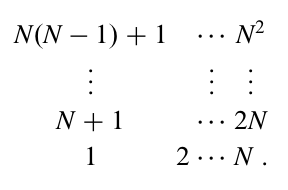
\includegraphics[scale=0.345]{arreglo1d}
\caption{Forma gráfica de visualizar una red de $N\times N$ en un arreglo 1-dimensional. Tomado de \cite{stickler} p. 238}
\end{figure}
\\
Para poder preservar la estructura de la red a pesar de estar en un contexto 1-dimensional, tenemos que generar una lista con los primeros vecinos del átomo i-ésimo, es decir una lista con el vecino de arriba, derecha, abajo e izquierda; todo ello considerando condiciones periódicas a la frontera, los pasos detallados para formar esta lista se encuentran en la sección \ref{apendice1}. Con esta lista de primeros vecinos podremos permitirnos calcular la energía de interacción que tiene el i-ésimo átomo con su entorno, la cual está dada por la ec. \ref{eq:Energia} que de manera discretizada la podemos visualizar como
\begin{equation}\label{eq:eDiscretizada}
\Delta E_{ij}=2J\sigma_{i,j}(\sigma_{i+1,j}+\sigma_{i-1,j}+\sigma_{i,j+1}+\sigma_{i,j-1})+2h\sigma_{i,j}
\end{equation}
para este caso vamos a considerar $h=0$. Notemos que lo que se encuentra entre paréntesis nos lo da directamente la lista de los primeros vecinos, por lo que esto nos facilita el cálculo de la energía de interacción del i-ésimo átomo. Posteriormente hay que definir la energía total del sistema sumando cada una de las energías para cada átomo de la red considerada, y la magnetización que no es más que la suma de todos los espines que existen en la configuración, es decir
\begin{align*}
E_{Total} &= \sum_i E_i,\qquad\text{donde $E_i$ es la energía del i-ésimo átomo}\\
\langle M\rangle &=\sum_i s_i,\qquad s_i\text{ el spín del i-ésimo átomo}
\end{align*}

\subsection{Temperatura crítica}
Para poder determinar la temperatura crítica es posible realizar una aproximación de campo medio \cite{tong} llegando a la ecuación trascendental
\begin{equation}\label{eq:trasc}
2\tanh^2\left(\frac{2J}{K_BT_C}\right)=1
\end{equation}
cuya solución para cierto valor de $J$ nos da la temperatura $T_C$ a la que ocurre la transición de fase de un ferromagneto a un paramagneto. Escogiendo $J=0.5$ y aplicando el algoritmo de Newton-Raphson para encontrar $T_C$, tenemos que tiene un valor aproximado de $T_C\approx 1.1346$.

\subsection{Termalización y Cantidades Observadas}\label{cantidadesObs}

Los recursos obtenidos hasta ahora son suficientes para poder proceder con el armado de Metrópolis para termalizar las configuraciones fría y caliente antes definidas, y determinar las cantidades observables. Recordemos que el proceso de termalización consiste en aplicar Metrópolis un determinado número de pasos hasta que la configuración sea aceptada y se pueda construir una cadena de Markov consistente, para ello se recomienda elegir un número grande de pasos, en este caso se ha elegido $n=100\, 000$ pasos.\\
\\
Para la función de \texttt{termalización} comenzamos pre alocando un par de vectores\footnote{Uno para la energía por iteración y otro para la Magnetización por iteración.} de ceros de longitud $n$ y aplicando un ciclo \texttt{for} desde uno hasta el número de pasos: se define la energía de una configuración arbitraria y se aplican las condiciones explicadas al inicio de esta sección; si se cumplen las condiciones se voltea el espín de la configuración y se pasa al siguiente paso con otra configuración; si no se cumplen entonces la configuración se rechaza y se pasa a una nueva. En cada iteración se va guardando la energía y magnetización total del sistema en los vectores pre alocados y así conseguimos termalizar las redes consideradas.\\
\\
Las cantidades observables se obtendrán únicamente para la configuración fría ya que es la que se asemeja a un ferromagnético y lo que queremos apreciar es su comportamiento conforme lo vamos calentando hacia su temperatura crítica; dichas cantidades observables devienen de la física estadística que de acuerdo a un cierto \cite{stickler} tratado las podemos expresar como
\begin{align}
\langle\epsilon\rangle&=\frac{\langle E\rangle}{N^2},\qquad\qquad\qquad\qquad \langle|m|\rangle=\frac{|\langle M\rangle|}{N^2}\label{eq:EyM}\\
C_H&=k_B\beta^2\left[\langle E^2\rangle-\langle E\rangle^2\right],\qquad \chi_m=\beta\left[\langle M^2\rangle-\langle M\rangle^2\right]\label{eq:CyX}
\end{align}
Para poder obtenerlas es muy sencillo, tenemos que modificar un poco la función de \texttt{termalización}. En lugar de que nos devuelva un vector con las energías y magnetización por iteración, le pediremos que nos devuelva la energía y magnetización final, es decir, la energía y magnetización total del último paso de la termalización. Posteriormente vamos a agarrar un conjunto de temperaturas comprendidas en el intervalo $T=[0,2.5]$ con un paso de $h=0.05$ y se construirá otra función de \texttt{cantidades observables} en donde termalizará la configuración fría para cada temperatura de $T$ obteniendo su respectiva energía y magnetización final. \\
\\
Si hacemos esto en principio deben salir resultados horrendos ya que el error asociado a las cantidades observables dados por integración Montecarlo va como $\approx\frac{1}{\sqrt{L}}$ donde en este caso $L$ es el número de termalizaciones que se hacen para una sola temperatura del conjunto considerado. En este caso se eligieron 400 termalizaciones ya que el error asociado sería de $0.05$. Por tanto, la función de \texttt{cantidades observables} va a tomar la energía y magnetización de las 400 termalizaciones y les aplicará un promedio para poder determinar la energía por sitio y la magnetización por sitio (ecs. \ref{eq:EyM}); para el calor específico y la susceptibilidad magnética se aplicará la varianza de la energía y la magnetización de las 400 termalizaciones (ecs. \ref{eq:CyX}), y todo ello para cada temperatura de $T$\footnote{En contraste con \texttt{termalización}, la función de \texttt{cantidades observables} pudo desempeñarse de manera óptima hasta $n=200\, 000$ pasos. Para más detalle, el código implementado en esta sección estará disponible en la sección \ref{apendice2}.}.


\section{Resultados}

\subsection{Proceso de termalización}

En esta primera sección de los resultados\footnote{Se utilizó la función \texttt{termalización}} se pretende estudiar el proceso de termalización desde dos perspectivas diferentes: analizando cómo es la energía y magnetización por iteración para dadas dos temperaturas $T_1<T_C$ y $T_2>T_C$; también se verán cómo son las configuraciones finales de una red de $N=100$ para 6 temperaturas distintas, es decir, la configuración más probable como resultado de termalizar el sistema $n=100\, 000$ pasos.\\
\\
\begin{figure}[h!]
\centering
	\subfloat[Energía por iteración.]{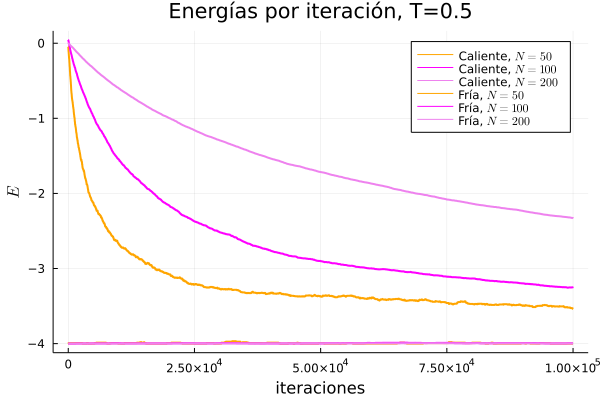
\includegraphics[scale=0.39]{energiaIteracionF}}
	\subfloat[Magnetización por iteración.]{
		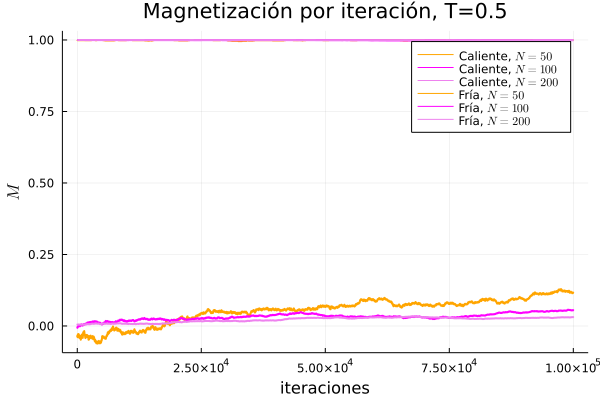
\includegraphics[scale=0.39]{magnIteracionF}}
\caption{Energía y magnetización por cada iteración para una temperatura $T=0.5$. Se consideraron $n=100\, 000$ pasos de termalización.}	
\label{fig:EM05}
\end{figure}

Las energías por iteración fueron tomadas a dos diferentes temperaturas, una menor a la temperatura crítica y otra mayor a la temperatura crítica con el fín de observar el contraste que hay en estas regiones, y de manera análoga se hizo lo mismo para la magnetización. Las redes consideradas en este proceso fueron de los tamaños $N=50,\, 100,\, 200$ y así mismo en cada gráfica se hace la distinción entre el comportamiento de la configuración fría y la caliente.

\begin{figure}[h!]
\centering
	\subfloat[Energías por iteración.]{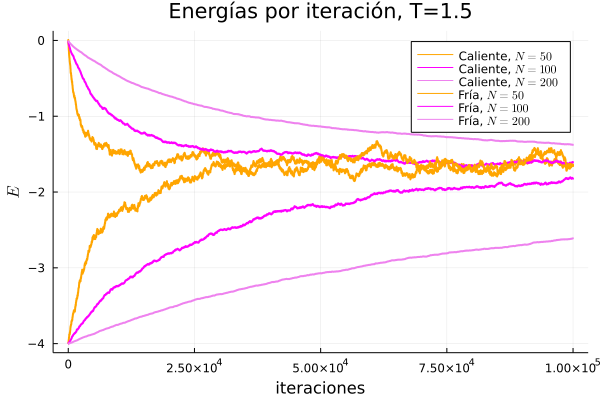
\includegraphics[scale=0.39]{energiaIteracionC}}
	\subfloat[Magnetización por iteración.]{
		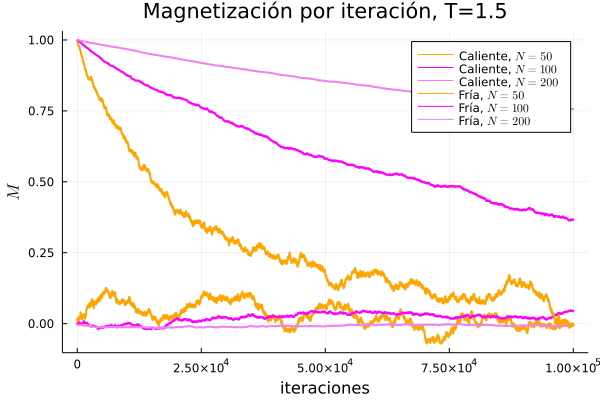
\includegraphics[scale=0.39]{magnIteracionC}}
\caption{Energía y magnetización por cada iteración para una temperatura $T=1.5$. Se consideraron $n=100\, 000$ pasos de termalización.}	
\label{fig:EM15}
\end{figure}
\newpage
Apreciando como es el comportamiento de las energías y magnetización por iteración, cabe preguntarse ¿cómo serían las configuraciones resultantes de espines previas y posteriores a la temperatura crítica? He aquí el resultado
\begin{figure}[h!]
\centering
\subfloat[$T=0.1$]{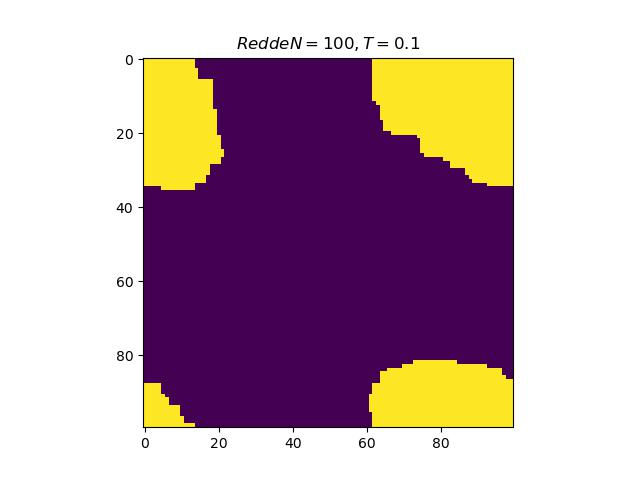
\includegraphics[scale=0.3]{T01}}
\subfloat[$T=0.5$]{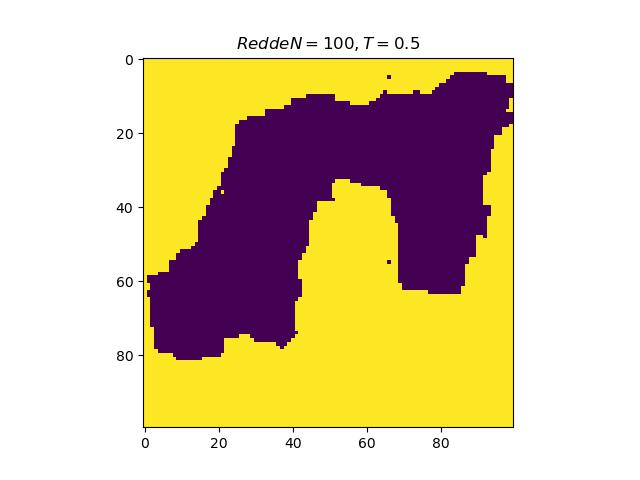
\includegraphics[scale=0.3]{T05}}
\subfloat[$T=1$]{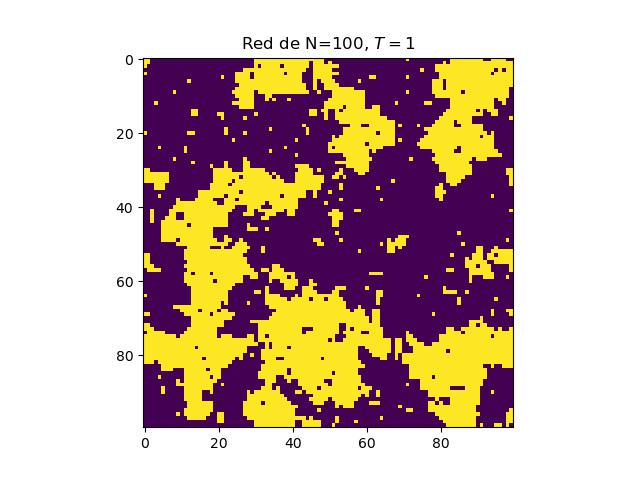
\includegraphics[scale=0.3]{T1}}\\
\subfloat[$T=T_C$]{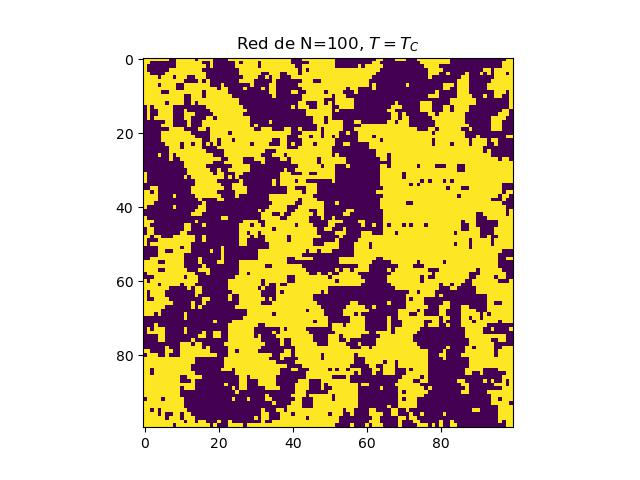
\includegraphics[scale=0.3]{TC}}
\subfloat[$T=1.5$]{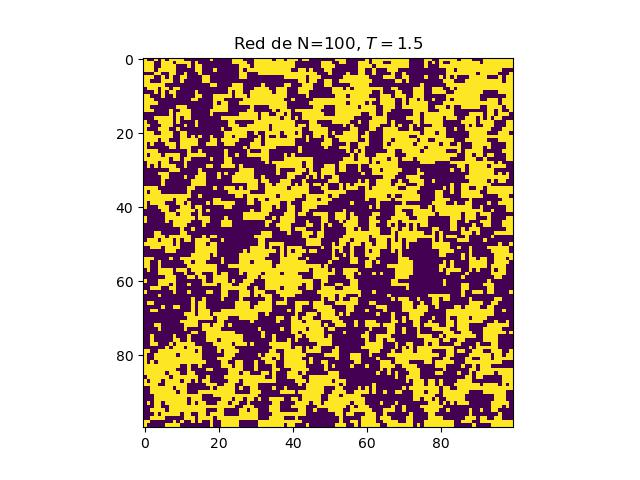
\includegraphics[scale=0.3]{T15}}
\subfloat[$T=2.5$]{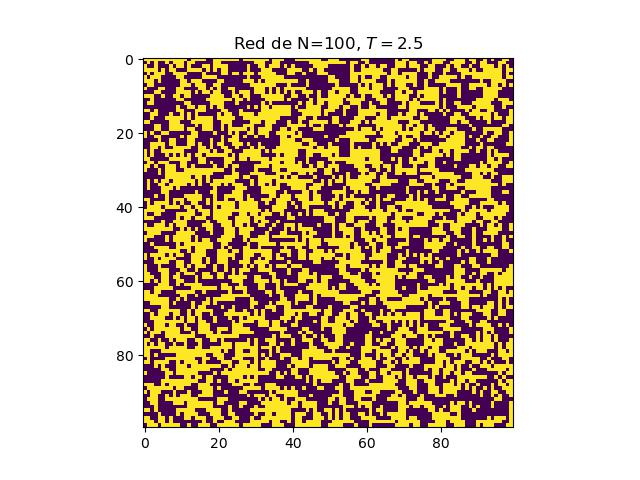
\includegraphics[scale=0.3]{T25}}
\caption{Configuraciones de $100\times 100$ espines resultantes de termializar el sistema $100\, 000$ veces para tres temperaturas menores a la temperatura crítica y tres temperaturas mayores o iguales a la temperatura crítica.}
\label{fig:confs}
\end{figure}

\subsection{Cantidades observables}

Las cantidades observables se determinaron a partir de la función \texttt{cantidades observables} discutida al final de la sección \ref{cantidadesObs}; se recuerda al lector que se escogió un intervalo de temperaturas $[0,2.5]$ con un paso de $h=0.05$. Para cada temperatura se termalizó 400 veces y se hicieron promedios para determinar cada cantidad observable
\begin{figure}[h!]
\centering
\subfloat[Energía por sitio]{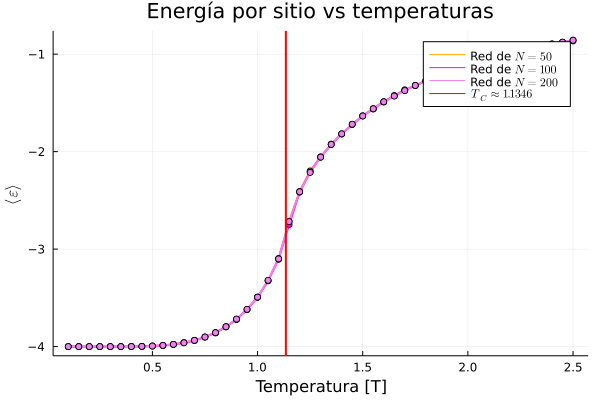
\includegraphics[scale=0.39]{enerSitio}}
\subfloat[Magnetización por sitio]{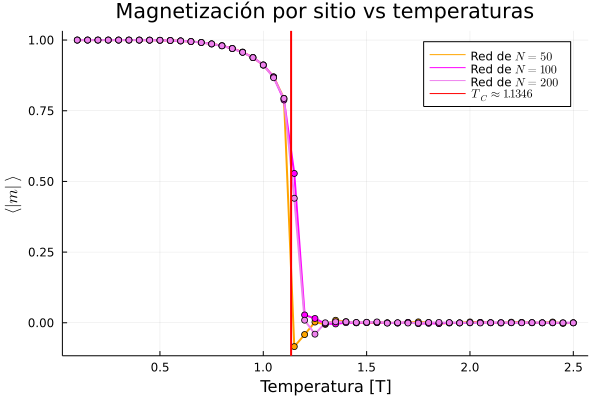
\includegraphics[scale=0.39]{magnSitio}}
\caption{Energía y Magnetización por sitio. Se consideraron $n=200\, 000$ pasos de termalización. }
\label{fig:eSymS}
\end{figure}
\newpage
En cada una de las cantidades observables se encuentra una línea vertical que representa la temperatura crítica. Es claro notar como existe un cambio de fase una vez que se cruza la $T_C$
\begin{figure}[h!]
\centering
\subfloat[Calor Específico]{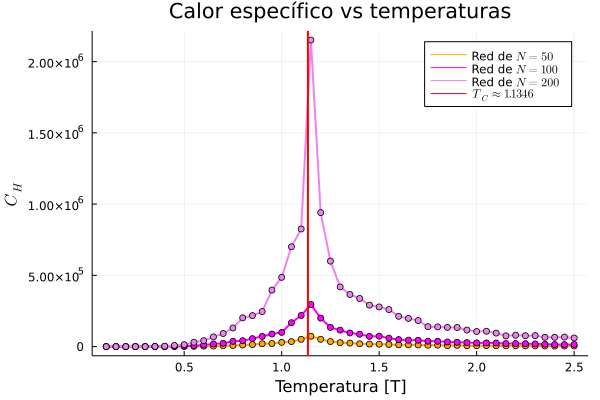
\includegraphics[scale=0.39]{calorEsp}}
\subfloat[Susceptibilidad magnética]{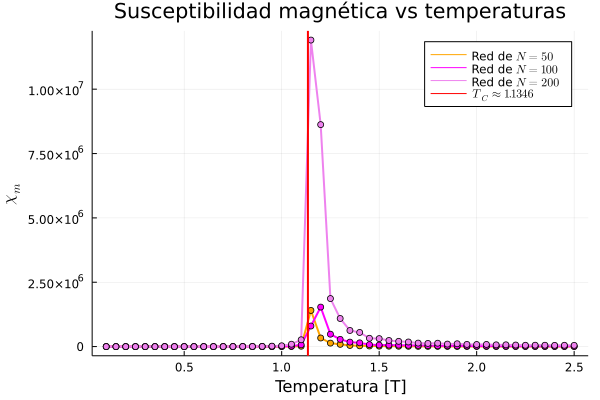
\includegraphics[scale=0.39]{susMag}}
\end{figure}

\section{Discusión}
\subsection{Proceso de termalización}

Para el caso de la energía y magnetización por iteración, podemos destacar que para temperaturas previas a la temperatura crítitca (fig. \ref{fig:EM05}) la energía de la configuración fría se queda más o menos constante (y es máxima) esto se debe a que las interacciones de espines del ferrromagneto son  tan fuertes que tiende a quedarse en su estado inicial, de hecho la magnetización para esta temperatura también es máxima; en contraste, la configuración caliente decae hacia un estado de máxima energía pero podemos observar como para cada red el decaimiento es distinto, siendo la de $50$  la que decae más rápido que la de $200$, esto en principio es debido a que le tomará más tiempo (pasos de termalización) en decaer a las redes grandes que a las pequeñas. Cada red caliente con el tiempo suficiente alcanzará a convertirse en una red fría, aunque esto es físicamente es imposible porque violaría la segunda ley de la termodinámica: un paramagneto no puede convertirse en un ferromagneto así de la nada.\\
\\
El chiste de la configuración caliente es más visible en la fig. \ref{fig:EM15}, lo que vemos es que ambas configuraciones (de cada red) tienden hacia un umbral de energías  cercanas entre sí para una temperatura superior a la crítica; en el caso de la configuración fría, tiende hacia un estado de mínima energía\footnote{avalada/abalada por la segunda ley de la termodinámica. *(chiste: garantizada y abalada)}. Por tanto la configuración caliente nos ayuda a visualizar de manera cualitativa la energía a la que debería topar la configuración fría debido al proceso de termalización. Por otro lado, la magnetización de la configuración fría tiende abruptamente hacia cero, tal y como se encuentra la configuración caliente; esto nos indica que un ferromagneto calentado a una temperatura mayor o igual a la crítica: pierde su propiedad de ferromagneto pasando a paramagneto.\\
\\
De la figura \ref{fig:confs} se destaca de manera visible como las interacciones entre espines en un ferromagneto son más fuertes para cuando estamos en régimen menor a la temperatura crítica. La fig. \ref{fig:confs}\textcolor{blue}{(d)} es una configuración a la que se le sometió la temperatura crítica y a partir de ese punto en adelante, (véase para $T=1.5$ y $T=2.5$) las interacciones son cada vez más débiles y por tanto el sistema no volverá a “ordenarse'' en los patrones que se observan previos a $T_C$, dicho de otra manera: el sistema no volverá a ser un ferromagneto sino que ha pasado a ser un paramagneto\footnote{a menos claro que se le vuelva a imponer un campo magnético que alinee los dominios magnéticos.}.

\subsection{Cantidades observables}

Las cantidades observables nos ayudarán a reforzar los argumentos manejados hasta ahora, es claro observar como existe una transición de fase para cada una de las cantidades observables. Previo y posterior a la temperatura crítica tenemos dos diferentes comportamientos para cada cantidad observable. Para la energía por sitio del ferromagneto es máxima para valores cercanos al cero y pasando $T_C$ tenemos un paramagneto con una energía que tenderá a cero conforme $T$ aumente, por otro lado pareciera que la temperatura crítica es un punto de inflexión en la energía por sitio, lo cual refuerza la idea de un cambio de fase. De la capacidad calorífica tenemos que en la temperatura crítica la energía necesaria para aumentar la temperatura del sólido cristalino  es alta a comparación de los alrededores en donde se ve como decrece. Lejos de la temperatura crítica, la capacidad calorífica es baja.\\
\\
Para el caso de la magnetización, ésta es máxima previa a la temperatura crítica y en el momento en que nos acercamos a ella tenemos un cambio abrupto decayendo a cero y pasando a un paramagneto. Sin embargo la magnetización por sitio es continua tal y como se discutió en la introducción; la manera de ver la transición de fase con esta cantidad observable: es mediante el cambio abrupto ocurrido en $T_C$. Por otro lado es completamente visible la discontinuidad de la susceptibilidad magnética dada por la ley de Curie-Wiess (ec. \ref{eq:Curie-Wiess}) recordemos que existe una discontinuidad en la segunda derivada de la energía con respecto del campo magnético, y esa discontinuidad la tenemos a la temperatura de Curie. La gráfica de la susceptibilidad magnética sugiere que en $T_C$ la susceptibilidad magnética tiende a infinito solo que la computadora nos devuelve numeros muy grandes, por lo que terminamos por mostrar que la transición de fase es de segundo orden. 
\section{Conclusiones}

El modelo de Ising es una herramienta clave en el estudio de las transiciones de fase en un ferromagneto. Por medio de las cantidades observables podemos observar este comportamiento e incluso se puede corroborar con la teoría cómo es que se trata de una transición de fase de segundo orden mediante la discontinuidad que presenta la susceptibilidad mangética; esta transición de fase lleva consigo una ruptura en la simetría de un ferromagneto pasando a un paramagneto en la temperatura crítica. El hecho de que la susceptibilidad magnética y el calor específico sean muy grandes cerca de la temperatura crítica demuestra que son máximas cerca de $T_C$, por lo que la energía necesaria para calentar el sólido cristalino y la susceptibilidad de que el material sea magnetizado por un campo magnético externo: son infinitas en $T_C$.\\
\\
Para agregar más sabor a este trabajo se recomienda considerar $h\neq0$ de la ec. \ref{eq:eDiscretizada} para ver que ocurre con las transiciones de fase en presencia de un campo magnético. 


\section{Apéndices}

\subsection{Apéndice A}\label{apendice1}

En esta sección se muestran los pasos detallados para formar la lista de los cuatro vecinos. Cada uno de ellos deberá cumplir una de dos condiciones de acuerdo al sitio del i-ésimo átomo de la lista
\begin{itemize}
\item[Arriba.] Si el sitio es $i\leq N^2$ entonces el vecino de arriba es igual a  $i+N$. Por otro lado si $i>N^2$ entonces el vecino de arriba es igual a $i-N(N-1)$.
\item[Derecha.] Si $\mod(i,N)\neq 0$, entonces el vecino de la derecha es $i+1$. En otro caso, el vecino de la derecha es igual a $i-N+1$.
\item[Abajo] Si el sitio es $i-N\geq 1$ entonces el vecino de abajo es $i-N$. En caso contrario el sitio de abajo es $i+N(N-1)$.
\item[Izquierda] Si $\mod(i-1,N)\neq 0$ entonces el vecino de la izquierda es $i-1$. En otro caso sería $i+N-1$
\end{itemize}



\subsection{Apéndice B}\label{apendice2}

Aquí se pueden encontrar las funciones más importantes. En una siguiente edición pondré el código completo y su explicación
\begin{figure}[h!]
\centering
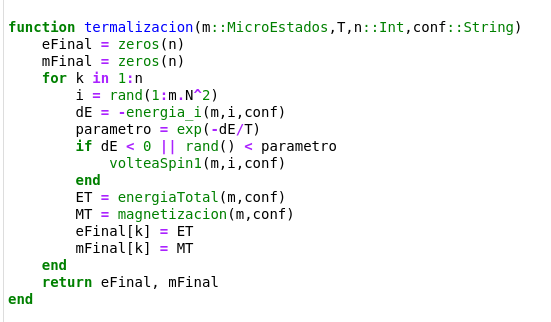
\includegraphics[scale=0.5]{1}
\caption{Función \texttt{termalización.}}
\end{figure}
\begin{figure}[h!]
\centering
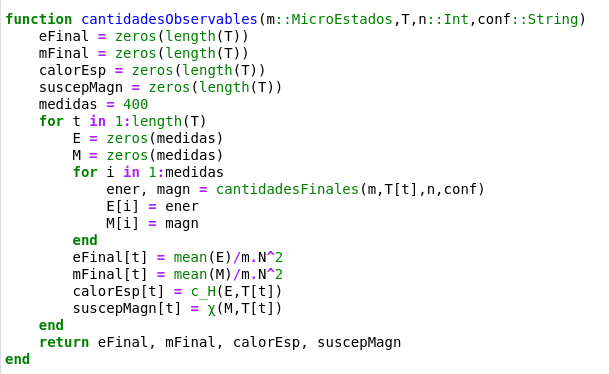
\includegraphics[scale=0.5]{2}
\caption{Función \texttt{cantidades observables.}}
\end{figure}


\begin{thebibliography}{9}
\bibitem{stickler} Stickler, Schachinger (2016) \emph{Basic Concepts in Computational Physics} Springer, 2ed.
\bibitem{tong} Tong, D. (2012) \textit{Statistical Physics}, University of Cambridge Part II Mathematical Tripos.

\bibitem{jack} Jackson, J. (1976) \textit{Classical Electrodynamics}, University of California, Berkley, 2ed.

\bibitem{hola} CoSIAM (21 septiembre, 2021) \textit{CoSIAM - Curso Corto - Introducción a la Modelación: 10. Algoritmo de Metrópolis.} \url{https://www.youtube.com/watch?v=aiPsbPxT29M&t=338s}

\end{thebibliography}

\end{document}